% ****************************************************************************************** % Dissertation template and document class for Princeton University
% Author  : Jeffrey Scott Dwoskin <jdwoskin@princeton.edu>
% Adapted from: http://www.math.princeton.edu/graduate/tex/puthesis.html
% ****************************************************************************************** %


%%% For print copies
%% set 'singlespace' option to set entire thesis to single space, and define "\printmode" to remove all hyperlinks for printed copies of the thesis. Delete all output files before changing this mode -- it will turn hyperref package on and off
%\documentclass[12pt,lot, lof, singlespace]{puthesis}
%\newcommand{\printmode}{}

%%% For the electronic copy, use doublespacing, define "\proquestmode" to use outlined links, instead of colored links. 
\documentclass[12pt,lot, lof]{puthesis}
\newcommand{\proquestmode}{}
% I prefer proquestmode to be off for electronic copies for normal use, since the colored links are less distracting. However when printed in black and white, the colored links are difficult to read. 

%%% For early drafts without some of the frontmatter
% Also see the "ifodd" command below to disable more frontmatter
%\documentclass[12pt]{puthesis}

%%%%%%%%%%%%%%%%%%%%%%%%%%%%%%%%%%%%%%%%%%%%%%%%%%%%%%%%%%%%%\
%%%% Author & title page info

\title{Particle Filter Localization for Unmanned Aerial Vehicles Using Augmented Reality Tags}

\submitted{May 2013}  % degree conferral date (January, April, June, September, or November)
\copyrightyear{2013}  % year in which the copyright is secured by publication of the dissertation.
\author{Edward Francis Kelley V}
\adviser{Professor Szymon Rusinkiewicz}  %replace with the full name of your adviser
%\departmentprefix{Program in}  % defaults to "Department of", but programs need to change this.
\department{Computer Science}

%%%%%%%%%%%%%%%%%%%%%%%%%%%%%%%%%%%%%%%%%%%%%%%%%%%%%%%%%%%%%\
%%%% Tweak float placements
% From: http://mintaka.sdsu.edu/GF/bibliog/latex/floats.html "Controlling LaTeX Floats"
% and based on: http://www.tex.ac.uk/cgi-bin/texfaq2html?label=floats
% LaTeX defaults listed at: http://people.cs.uu.nl/piet/floats/node1.html

% Alter some LaTeX defaults for better treatment of figures:
    % See p.105 of "TeX Unbound" for suggested values.
    % See pp. 199-200 of Lamport's "LaTeX" book for details.
    %   General parameters, for ALL pages:
    \renewcommand{\topfraction}{0.85}	% max fraction of floats at top
    \renewcommand{\bottomfraction}{0.6}	% max fraction of floats at bottom
    %   Parameters for TEXT pages (not float pages):
    \setcounter{topnumber}{2}
    \setcounter{bottomnumber}{2}
    \setcounter{totalnumber}{4}     % 2 may work better
    \setcounter{dbltopnumber}{2}    % for 2-column pages
    \renewcommand{\dbltopfraction}{0.66}	% fit big float above 2-col. text
    \renewcommand{\textfraction}{0.15}	% allow minimal text w. figs
    %   Parameters for FLOAT pages (not text pages):
    \renewcommand{\floatpagefraction}{0.66}	% require fuller float pages
	% N.B.: floatpagefraction MUST be less than topfraction !!
    \renewcommand{\dblfloatpagefraction}{0.66}	% require fuller float pages

% The documentclass already sets parameters to make a high penalty for widows and orphans. 

%%%%%%%%%%%%%%%%%%%%%%%%%%%%%%%%%%%%%%%%%%%%%%%%%%%%%%%%%%%%%\
%%%% Use packages

%\usepackage{amsfonts}

%%% For figures
\usepackage{graphicx}
\usepackage{caption}
\usepackage{subcaption}
\usepackage{amsmath}
% \usepackage{subfig,rotate}

%%% for comments
\usepackage{verbatim}

%%% For tables
\usepackage{multirow}
% Longtable lets you have tables that span multiple pages.
\usepackage{longtable}

% Booktabs produces far nicer tables than the standard LaTeX tables.
%   see: http://en.wikibooks.org/wiki/LaTeX/Tables
\usepackage{booktabs}

\usepackage{listings}

\singlespacing
\usepackage{color}
\usepackage{listings}
\lstset{ %
language=Python,                % choose the language of the code
basicstyle=\footnotesize,       % the size of the fonts that are used for the code
numbers=left,                   % where to put the line-numbers
numberstyle=\footnotesize,      % the size of the fonts that are used for the line-numbers
stepnumber=1,                   % the step between two line-numbers. If it is 1 each line will be numbered
numbersep=8pt,                  % how far the line-numbers are from the code
backgroundcolor=\color{white},  % choose the background color. You must add \usepackage{color}
showspaces=false,               % show spaces adding particular underscores
showstringspaces=false,         % underline spaces within strings
showtabs=false,                 % show tabs within strings adding particular underscores
tabsize=2,          % sets default tabsize to 2 spaces
captionpos=b,           % sets the caption-position to bottom
breaklines=true,        % sets automatic line breaking
breakatwhitespace=false,    % sets if automatic breaks should only happen at whitespace
escapeinside={\%*}{*)}          % if you want to add a comment within your code
}

%set parameters for longtable:
% default caption width is 4in for longtable, but wider for normal tables
\setlength{\LTcapwidth}{\textwidth}



%%%%%%%%%%%%%%%%%%%%%%%%%%%%%%%%%%%%%%%%%%%%%%%%%%%%%%%%%%
%%% Printed vs. online formatting
\ifdefined\printmode

% Printed copy
% url package understands urls (with proper line-breaks) without hyperlinking them
\usepackage{url}


\else

\ifdefined\proquestmode
%ProQuest copy -- http://www.princeton.edu/~mudd/thesis/Submissionguide.pdf

% ProQuest requires a double spaced version (set previously). They will take an electronic copy, so we want links in the pdf, but also copies may be printed or made into microfilm in black and white, so we want outlined links instead of colored links.
\usepackage{hyperref}
\hypersetup{bookmarksnumbered}

% copy the already-set title and author to use in the pdf properties
\makeatletter
\hypersetup{pdftitle=\@title,pdfauthor=\@author}
\makeatother

\else
% Online copy

% adds internal linked references, pdf bookmarks, etc

% turn all references and citations into hyperlinks:
%  -- not for printed copies
% -- automatically includes url package
% options:
%   colorlinks makes links by coloring the text instead of putting a rectangle around the text.
\usepackage{hyperref}
\hypersetup{colorlinks,bookmarksnumbered}

% copy the already-set title and author to use in the pdf properties
\makeatletter
\hypersetup{pdftitle=\@title,pdfauthor=\@author}
\makeatother

% make the page number rather than the text be the link for ToC entries
%\hypersetup{linktocpage}
\fi % proquest or online formatting
\fi % printed or online formatting


%%%%%%%%%%%%%%%%%%%%%%%%%%%%%%%%%%%%%%%%%%%%%%%%%%%%%%%%%%%%%\
%%%% Define commands

% Define any custom commands that you want to use.
% For example, highlight notes for future edits to the thesis
%\newcommand{\todo}[1]{\textbf{\emph{TODO:}#1}}

% create an environment that will indent text
% see: http://latex.computersci.org/Reference/ListEnvironments
% 	\raggedright makes them left aligned instead of justified
\newenvironment{indenttext}{
    \begin{list}{}{ \itemsep 0in \itemindent 0in
    \labelsep 0in \labelwidth 0in
    \listparindent 0in
    \topsep 0in \partopsep 0in \parskip 0in \parsep 0in
    \leftmargin 1em \rightmargin 0in
    \raggedright
    }
    \item
  }
  {\end{list}}

% another environment that's an indented list, with no spaces between items -- if we want multiple items/lines. Useful in tables. Use \item inside the environment.
% 	\raggedright makes them left aligned instead of justified
\newenvironment{indentlist}{
    \begin{list}{}{ \itemsep 0in \itemindent 0in
    \labelsep 0in \labelwidth 0in
    \listparindent 0in
    \topsep 0in \partopsep 0in \parskip 0in \parsep 0in
    \leftmargin 1em \rightmargin 0in
    \raggedright
    }

  }
  {\end{list}}



%%%%%%%%%%%%%%%%%%%%%%%%%%%%%%%%%%%%%%%%%%%%%%%%%%%%%%%%%%%%%\
%%%% Front-matter

% For early drafts, you may want to disable some of the frontmatter. Simply change this to "\ifodd 1" to do so.
\ifodd 0
% front-matter disabled while writing chapters
\renewcommand{\maketitlepage}{}
\renewcommand*{\makecopyrightpage}{}
\renewcommand*{\makeabstract}{}

% you can just skip the \acknowledgements and \dedication commands to leave out these sections.

\else


\abstract{
% Abstract can be any length, but should be max 350 words for a Dissertation for ProQuest's print indicies (150 words for a Master's Thesis) or it will be truncated for those uses.
This paper proposes a system for capturing 3D imagery of large objects using autonomous quadcopters. A major component of such a system is accurately localizing the position and orientation of the quadcopter in order to perform precise movements. This paper focuses on the design and implementation of a localization algorithm that uses a particle filter to combine internal sensor measurements and detected augmented reality tags in order to estimate the position and orientation of an AR.Drone quadcopter. This system is shown to perform significantly better than integrated velocity measurements alone.
}

\acknowledgements{
%I would like to thank...
Completing this thesis has been one of the most challenging, yet fulfilling experiences I have had in my time here at Princeton. I could never have completed this alone and I am indebted to a long list of mentors, friends, and family.

First and foremost, I would like to express my gratitude to my advisor, Szymon Rusinkiewicz, whose support and advice has been invaluable throughout this entire process. Professor Rusinkiewicz went above and beyond what could be expected of an undergraduate thesis advisor and I appreciate how much I have learned from him, ever since my days of struggling through ``Death Graphics.'' I would also like to thank Professor Robert Stengel for his advice and support, as well as Professor Christopher Clark for introducing me to robotics and continuing to be a valuable source of advice during this project.

Furthermore, this project was funded by the School of Engineering and Applied Science, as well as the Morgan McKinzie $'$93 Senior Thesis Prize Fund. I am grateful to attend a school that makes projects such as this possible.

A special thanks goes to my thesis partner Sarah Tang. Her friendship and cheery disposition made those long hours of watching generally-uncooperative quadcopters a fun and memorable experience.

I would also like to thank everyone who made my time at Princeton incredible. In particular: my fellow hashers in the Princeton Tower Club for keeping my spirits up and providing wonderful distractions from my computer screen; my quasi-roommates and dinner companions, Nick Adkins and Alice Fuller, for bringing me so much happiness and laughter; John Subosits for indulging my pretending to be an engineer; Rodrigo and the rest of the Menezes family for claiming me as one of their own; Jonathan Yergler, Coach Zoltan Dudas, and the rest of the Princeton Fencing Team for all of the wonderful memories, both on and off the strip.

Finally, I would like to thank my parents. It is only with their love and support that I have made it to this point. I am unable to fully convey my appreciation for everything they have done.


}
\dedication{To my parents.}
\honorcode{\textit{This thesis represents my own work in accordance with University regulations.}}

\fi  % disable frontmatter

\newcommand{\degree}{\ensuremath{^\circ~}}

\usepackage{url}
\usepackage{algpseudocode}
\usepackage{algorithm}

\begin{document}

\makefrontmatter


% If you've disabled frontmatter, you can insert the toc manually
%\tableofcontents\clearpage

% \include lets us split up the document (and each include starts a new page):

\chapter{Introduction\label{ch:intro}}

% Talk about the increasing use of quadcopters for a variety of uses.
In recent years, research using small-scale Unmanned Aerial Vehicles (UAVs) has increased rapidly. Multi rotor aircraft, such as quadcopters (also known as quadrotors), have proven to be powerful platforms for applications in a variety of fields, from aerial photography to search and rescue~\cite{Irschara, Gupte}. Once prohibitively expensive for most research projects, multi rotor aircraft have decreased substantially in price, ranging from a few hundred dollars to several thousand dollars. Additionally, on-board control systems have greatly added to the stability and ease of control of these aircraft, with many quadcopters using pre-programmed routines for difficult procedures such as takeoff and landing.


%Slightly repetitive. Also should this be in the related work section? What is the best way to split this up?
Although quadcopters have seen interest from the military and hobbyists for quite some time, these recent developments in price and stability have resulted in quadcopters being used in a wide array of applications. In 2010, a French company, Parrot, released the AR.Drone, a quadcopter intended for consumers. Unlike most other quadcopters, which were sold in kits targeted to experienced hobbyists or researchers, the AR.Drone was designed to be ready to fly right out of the box by an inexperienced pilot. Although affordable and easy to use, these quadcopters are far from just toys. Equipped with an array sensors and multiple cameras, the AR.Drone and other consumer-grade vehicles have been used by research groups to explore autonomous flight with a low barrier of entry, both in cost and complexity.

With the democratization of this technology, quadcopters can be used to be solved problems where cost and complexity for such a solution was once prohibitive.

\section{Motivation}

For applications ranging from developing video games to preserving archaeological artifacts, capturing 3D models of real-world objects has become an important task in a wide variety of fields. %Talk more about why 3D is important 

While there are currently several different methods for capturing these models, each of these methods has associated limitations and drawbacks.


\section{Current Acquisition Methods}

\subsection{Manual Model Creation}
The most common method of model acquisition is having a trained modeler produce a 3D model using reference imagery and measurements. Models are tediously crafted in CAD software in a process similar to sculpting. While this technique is used extensively in video games and films, it is typically too time consuming and expensive for many applications such as archeology.

\subsection{Laser Scanners}
Laser rangefinder technology is the ``gold standard'' of 3D model acquisition in terms of precision. Modern scanners can produce sub millimeter scans, which make them a great choice for detailed digitization of statues. Combined with high-resolution photograph texture-mapping, very few techniques can match the precision and quality of these scans. The Digital Michelangelo Project showed the power and precision of laser scanners by scanning several different statues, including Michelangelo's David, to 1/4mm accuracy~\cite{Levoy}.

\begin{figure}
\centering
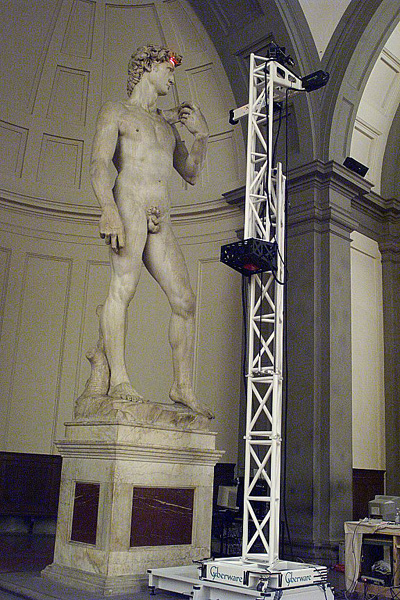
\includegraphics[height=200px]{../images/david_scan.jpg}
\caption{An example of a laser scanner setup used by the Digital Michelangelo Project~\cite{Levoy}.}
\end{figure}

However, laser scanners do have several drawbacks. The equipment is extremely expensive, bulky, and fragile. The Michelangelo Project had to transport over 4 tons of equipment to Italy in order to produce their scans. Additionally, laser scans involve immense setup and can take many hours. The model of David took over a thousand man-hours to scan and even more than that in post processing~\cite{Levoy}.

\subsection{Multi-View Stereo}
Multi-view stereo uses a collection of 2D images to reconstruct a 3D object model. By viewing a single object from hundreds of different camera positions, it is possible to generate a 3D model. Although this technique originally required precisely known camera coordinates, recent algorithms can produce a 3D model from an unordered collection of images with unknown camera positions, assuming that there is sufficient coverage. Existing software packages such as Bundler and Agisoft Photoscan can produce high-quality 3D reconstructions using these unordered image collections~\cite{bundler, Agisoft}.

The ability to use a collection of images without precise camera position information means that these 3D objects can be modeled substantially faster than with a laser scanner. With a smaller object, it is a relatively simple process to take pictures of the object from many different angles. However, for a larger object, such as a statue or building, the task of gathering imagery becomes substantially more difficult.

\begin{figure}
\centering
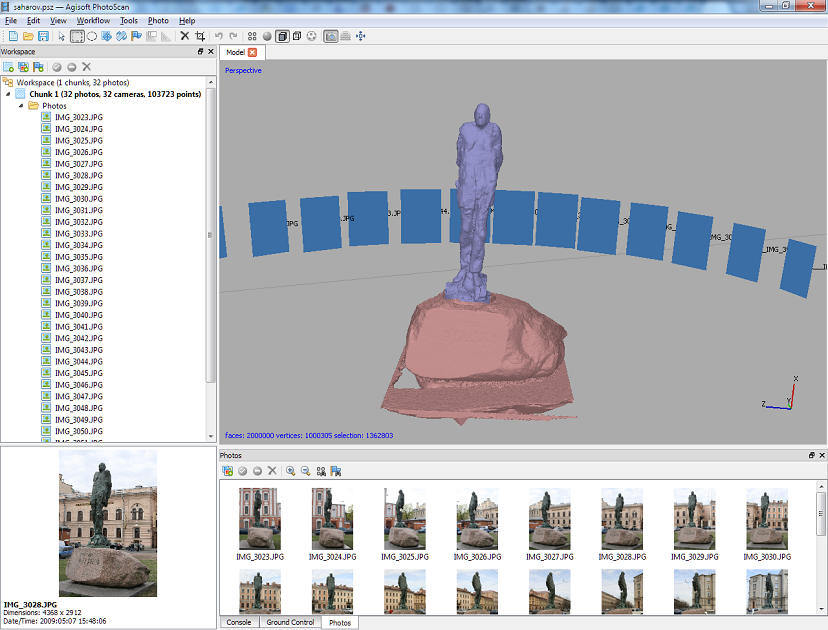
\includegraphics[height=200px]{../images/photoscan.png}
\caption{A 3D model of a statue generated by Agisoft Photoscan. Notice the derived camera planes encompassing the statue~\cite{Agisoft}.}
\end{figure}

\subsection{Microsoft Kinect}

Several groups have researched using the Microsoft Kinect for model acquisition. As the Kinect produces an RGB image with depth information, either the Kinect or the model most be moved in order to produce a complete scan. While this has been found to be useful in scanning small to medium size objects, such as people, the Kinect has several limitations. First of all, the depth range is rather short, on the order of a few meters. Additionally, because the depth is partially determined using an infrared pattern, the Kinect does not work in locations with a large amount of background infrared light, such as outdoors.


\section{Problem Definition}
The goal of this system to capture imagery of large 3D objects for use in multi-view stereo software. This system has several requirements:

\begin{enumerate}
\item
\textbf{Low Cost}

The system should be substantially cheaper than laser scanning.

\item
\textbf{Easy to Use}

This system should be able to be deployed by users with minimal training and setup. Additionally, the hardware should be off-the-shelf and easily accessible.

\item
\textbf{Complete Coverage}

The system must be able to capture images from a wide variety of positions, completely covering every part of the target object.

\item
\textbf{High Quality Imagery}

The system must produce sufficiently high resolution, non-blurry images for use in multi-view stereo software.

\end{enumerate}

\section{Proposed Solution}

We propose using low-cost autonomous quadcopters to gather the imagery needed for use in multi-view stereo software. By flying a quadcopter with a mounted camera around the target object, imagery can quickly be gathered from a wide variety of positions around the object. Using quadcopters has many advantages.

\begin{figure}
\centering
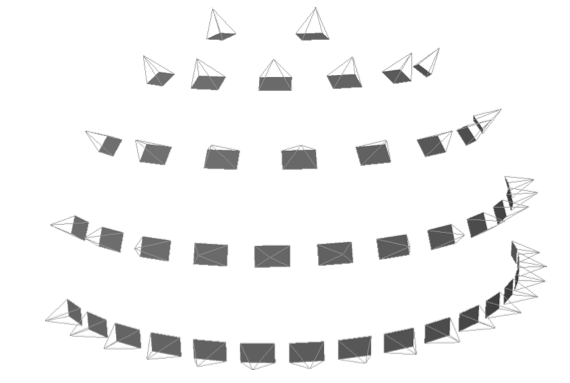
\includegraphics[width=200px]{../images/camera_network.png}
\caption{An example of camera positions for use in multi-view stereo. Such viewpoints could be attained by using quadcopters~\cite{Irschara}.}
\end{figure}

\begin{enumerate}
\item
Quadcopters can capture images from positions unreachable by ground-based cameras.

\item
By methodically flying around the target object at different altitudes, complete coverage of the target object can be achieved.

\item
The imagery can be captured very quickly, on the order of a few minutes.

\item
Quadcopters are small, portable, and easily deployable.


\end{enumerate}

\section{Solution Components}

In order to implement such a solution, there are two main components which must be created. First, a localization algorithm is needed to produce position and orientation estimates of the quadcopter in the global frame. Then, a controller is needed to produce the control inputs for the quadcopter to move in the desired path. This thesis focuses on the design, implementation, and testing of the localization component, while the thesis of Sarah Tang in the Mechanical and Aerospace Engineering Department addresses the controller component of this system.








\chapter{Related Work\label{ch:pastwork}}

This is related work.



\chapter{System Design\label{ch:system}}

\section{Parrot AR.Drone 2.0}

\section{System Architecture}

\subsection{Robot Operating System}

\subsection{ARDrone Autonomy}

\subsection{AR Toolkit}

\subsection{Localization}

\subsection{Controller}

\subsection{Agisoft Photoscan}



\chapter{Localization\label{ch:localization}}

\section{Problem Description}
	For a robot to perform precise maneuvers, it must first have an understanding of its position and orientation, or pose. This is the problem of localization. By using a variety of sensor measurements, the localization algorithm must produce a single estimate of the quadcopter's pose for use in the controller.

\section{Considerations of the AR.Drone}

	As this project uses the AR.Drone 2.0, the localization algorithm is built around the capabilities and limitations of this hardware. Considering the low load-capacity of the AR.Drone and the fact that this project aims to use off-the-shelf hardware, the localization algorithm may only use the sensors included in the AR.Drone.

	Therefore, the localization must produce an estimate by using some combination of the forward camera, downward camera, accelerometer, gyroscope, magnetometer, ultrasound altimeter, and pressure altimeter. 

\section{Localization Methods}

	Localization for mobile robots fall into three main categories: Kalman, Grid-Based, and Monte Carlo.

	%ASK: How do Kalman filters work?
	\subsection{Extended Kalman Filter}
	The extended Kalman Filter (EKF) is used extensively in mobile robot localization. The EKF is a nonlinear version of the Discrete Kalman Filter first introduced by Rudolf Emil Kalman in 1960~\cite{Kalman}. The EKF linearizes about the current mean and covariance in  method similar to a Taylor series. The EKF contains two stages, a prediction step and a correction step. In the prediction step, the new state and error covariance are projected. Then, in the correction step, the estimate and error covariance are updated in response to sensor measurements~\cite{Welch}. However, Kalman filters have the disadvantage of only being able to approximate normal distributions.

	%I need a better reason why I am not using Kalman filter
	\subsection{Grid-Based Markov Localization}
	Grid-based localization uses a ``fine grained'' grid approximation of the belief space, that is the space that covers all of the potential position and orientations of the robot~\cite{Fox}. For each time step, the probability of a robot being in any one of the grid cells is calculated, first by using odometry and then by exteroceptive sensors such as range finders. While relatively straightforward to implement, this process has many drawbacks. First of all, picking the size of the grid cells can be difficult. If the cells are too large, then the estimate will not be precise. However, if the cells are too small, the algorithm will be slow and very memory-intensive. Additionally, grid-based localization performs poorly in higher-dimensional spaces, as the number of cells grows exponentially with the number of dimensions.

	\subsection{Particle Filter}
	A particle filter is a type of Monte Carlo simulation with sequential importance sampling~\cite{Alkhatib}. Essentially, a particle filter keeps track of a large number of particles, which represent possible pose estimation. The particle filter typically moves these particles using proprioceptive sensor measurements convolved with Gaussian noise~\cite{Fox}. Then, the particles are weighted with respect to exteroceptive sensor measurements. These particles are then randomly resampled based on these weight values, producing a corrected distribution of particles.

	There are many advantages to using a particle filter. Due to the way the process creates an approximation by a set of weighted samples without any explicit assumptions of the approximation's form, it can be used in applications where the assumption of Gaussian noise doesn't necessarily apply~\cite{Alkhatib}.

\section{Particle Filter with Augmented Reality Tags}

	\begin{algorithm}
		\centering
		\caption{Particle Filter with Augmented Reality Tag Correction} 
		\begin{algorithmic}[1]
			\ForAll {$t$}
				\If{\textit{buffer\_full()}}
					\State{\textit{predict}$(\Delta t, v_x, v_y, altd, \theta)$}
				\EndIf
				\If{$recieved\_tag()$}
					\State {\textit{correct}$(\textbf{P})$} \Comment{Transformation matrix from camera to marker}
				\EndIf
				\State {$\textbf{x}_{est} \gets $\textit{get\_estimate()}}
			\EndFor
		\end{algorithmic}
	\end{algorithm}

	%Provide a brief background on the origination of the particle filter, uses, advantages, etc.
	The particle filter has been chosen for this project due to its flexibility, ease of implementation, and performance. In typical implementations of particle filters for mobile robots, the prediction step uses proprioceptive sensors, such as accelerometers, gyroscopes, and rotary encoders. Then, this estimate is typically corrected by using exteroceptive sensors, such as infrared, laser, or ultrasound.

	However, due to the lack of horizontal range sensing, this particle filter uses a different division between the prediction and correction steps. The prediction step uses the stock configuration of sensors in the AR.Drone, specifically the fused velocity, gyroscope, and ultrasound altimeter measurements. Then, the correction step uses an estimated global position determined by augmented reality tags to resample the particles.


	\subsection{Buffering Navdata}

		The localization module receives navdata at 50Hz. Depending on the number of particles and computational resources available to the localization algorithm, this can be a higher rate than the particle filter can run the propagation step. Reducing the rate at which propagation is run allows the particle filter to use more particles, providing better coverage of the pose estimate space and increasing the likelihood of convergence.

		Additionally, while a more rapidly updated pose estimate would be preferable, the accuracy of the measurement is not such that it is especially useful to update at a rate of 50Hz. For example, the maximum velocity that the quadcopter should ever achieve in this system is around 500mm/s. In .02 seconds, the quadcopter will have only moved 10mm, or 1cm. Considering that the desired accuracy of the localization is on the order of tens of centimeters, updating the estimated pose at a reduced rate is acceptable.

		As the navdata is recieved, the navdata measurements, such as velocity and yaw, are added to a buffer of size $n$. Every $n$ measurements, the propagate step is called with the simple moving average of the previous $n$ values and the sum of the $\Delta T$ values since the last call to propagate. This results in a propagate rate of $50/n$Hz.

		Although the buffer size is currently a hard-coded value, this could be dynamically changed based on the amount of delay between receiving navdata measurements and processing them in the propagate step. This would result in the highest propagate rate possible given a fixed number of particles. On the other hand, the buffer size could remain fixed with the particle filter adjusting the total number of particles, allowing for the best possible coverage at a guaranteed update rate.

	\subsection{Initialization}

		The particle filter is initialized by creating a set of $N$ particles. Each of these particles represents a potential pose in the configuration space. In particular, each particle at a given time step $t$ is of the form:

		\[\textbf{x}_t = \begin{bmatrix} 
			  x_t\\
			  y_t\\
			  z_t\\
			  \theta_t\\
			\end{bmatrix}	
		\]

		Where $x_t, y_t, z_t$ are the position, in mm, and $\theta_t$ is the heading, in degrees, of the particle in the global coordinate space. As the low level stabilization and control of the quadcopter is handled by the on-board processor, it is not necessary to include roll and pitch in the pose estimate of the quadcopter as these are not needed for the high level control. The entire set of particles of size $N$ at time step $t$ can be described as:

		\[
		\textbf{X}_t = [\textbf{x}_t[0], \textbf{x}_t[1],...,\textbf{x}_t[N]]^T
		\]

		Additionally, for each time step, there is a set of associated weights

		\[
		\textbf{W}_t = [w_t[0], w_t[1],...,w_t[N]]^T
		\]

		Normalized, such that

		\[
		\sum_{i=0}^N w_t[i] = 1
		\]


		\subsubsection{Coordinate Frame Conventions}

			\begin{figure}
			\centering
				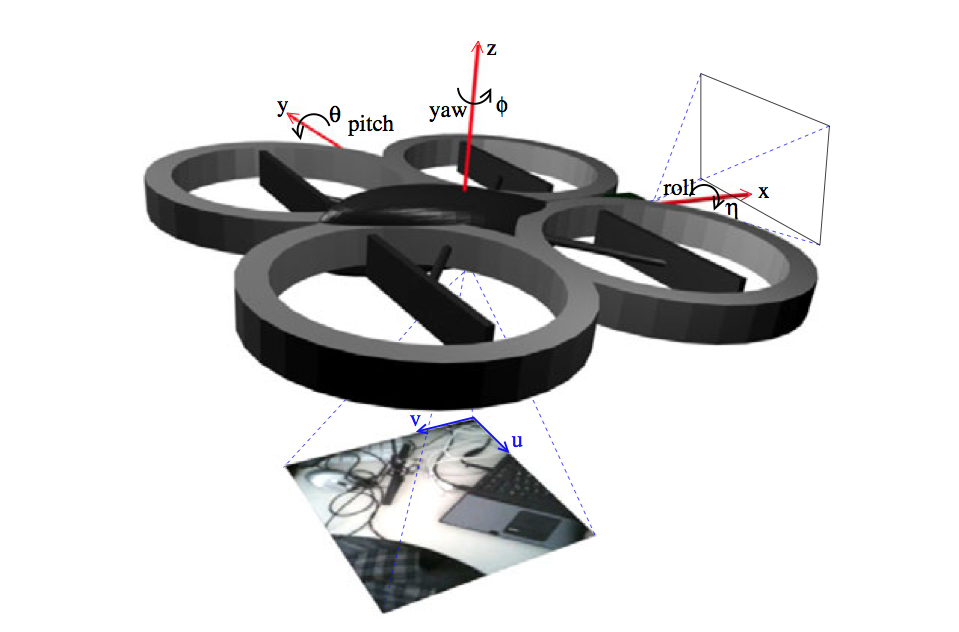
\includegraphics[width=300px]{../images/coordinates.png}
				\caption{AR.Drone Coordinate System~\cite{ARDroneEducation}.}\label{fig:coords}
			\end{figure}

			The coordinate frame follows the standard set by the ardrone\_autonomy package. As shown in Figure~\ref{fig:coords}, the coordinate frame is right-handed, with positive $x$ as forward, positive $y$ as left, and positive $z$ as up. In terms of rotation, a counter clockwise rotation about an axis is positive. Heading ranges from -180 degrees to 180 degrees, with 0 centered along the $x$-axis. When the particle filter is initialized, the global coordinate frame is set equal to the first instance of the local coordinate frame.


	\subsection{Prediction Step}

		\begin{algorithm}
			\centering
			\caption{Prediction Step} 
			\begin{algorithmic}[1]
				\Function{Predict}{$\Delta t, v_x, v_y, \theta, z_{\textit{ultra}}$}
					\State {$\Delta\theta \gets \theta -  \theta_{t-1}$}
					\For {$i=0 \to N$}
						\State {$\Delta\theta_{\textit{noise}} \gets \textit{randn}(\Delta\theta, \sigma_{\theta})$} 
						% \Comment{$randn(\mu, \sigma)$ returns a normally-distributed random value}
						\State {$\theta_{t}[i] \gets  \theta_{t-1}[i] + \Delta\theta_{\textit{noisy}}$} \label{predict:line:theta}
						\State {$(v_{\textit{x,global}} , v_{\textit{y,global}}) \gets \textit{transform}(v_x, v_y, \theta_{t}[i])$} \label{predict:line:transform}
						\State {$v_{\textit{x,global,noisy}} \gets \textit{randn}(v_{\textit{x,global}}, \sigma_{v})$}
						\State {$v_{\textit{y,global,noisy}} \gets \textit{randn}(v_{y,global}, \sigma_{v})$}
						\State {$x_{t}[i] \gets \Delta t*v_{\textit{x, global, noise}} + x_{t-1}[i]$} \label{predict:line:position}
						\State {$y_{t}[i] \gets \Delta t*v_{\textit{y, global, noise}} + y_{t-1}[i]$}
						\State {$z_{t}[i] \gets \textit{randn}(z_{\textit{ultra}}, \sigma_{ultra})$}
					\EndFor
				\EndFunction
			\end{algorithmic}
		\end{algorithm}

		The first component of a particle filter is the prediction step. In this step, the position of every particle is updated by using the sensor measurements contained in the navdata messages. Specifically, the prediction step uses the elapsed time, $\Delta t$, fused velocity measurements, $v_x$ and $v_y$, yaw reading, $\theta$, and ultrasound altimeter value, $z_{ultra}$.

		The prediction step then subtracts the value of $\theta_{t-1}$, the value of theta from the previous estimate, from $\theta$ to produce $\Delta\theta$. Then, for every particle $i$, a new pose $\textbf{x}_t[i]$ is generated using the previous pose, $\textbf{x}_{t-1}[i]$ and the values $\Delta t, v_x, v_y, \Delta\theta,$ and $z_{ultra}$.

		\subsubsection{Adding Noise to Sensor Measurements}
			In order to update the pose estimation for a given particle, noise is first added to the sensor measurements in order to model the sensor noise. By adding noise to the particles, the distribution of particles should expand to include all of the possible belief states.

			%INCLUDE A GRAPHIC SHOWING THE SPREADING OUT OF PARTICLES OVER TIME

			For each sensor value, a new ``noisy'' value is generating by a sampling from a Gaussian distribution with a mean of the sensor reading and a standard deviation, $\sigma$, which models in accuracy of the sensor. 
		
		\subsubsection{Converting Local Velocity to Global Velocity}
			In order to update the pose of each particle in the global frame, the values $v_{\textit{x,noisy}}$ and $v_{\textit{y,noisy}}$, must be transformed from the local coordinate frame of the quadcopter to the global coordinate frame. First, on Line~\ref{predict:line:theta}, the new heading of the particle is determined by adding the value $\Delta\theta_{\textit{noisy}}$ to the estimated heading of the last time step, $\theta_{t-1}[i]$.

			Then, on Line~\ref{predict:line:transform}, the global velocity is found by
			\[
			\begin{bmatrix} 
			  v_{\textit{x,global,noisy}}\\
			  v_{\textit{y,global,noisy}}\\
			\end{bmatrix}
			=
			\begin{bmatrix} 
			  cos(\theta_t[i]) & -sin(\theta_t[i])\\
			  sin(\theta_t[i]) & cos(\theta_t[i])\\
			\end{bmatrix}
			\begin{bmatrix} 
			  v_{\textit{x,noisy}}\\
			  v_{\textit{y,noisy}}\\
			\end{bmatrix}
			\]

		\subsubsection{Position Update}
			Once the velocity is in the global coordinate frame, Euler integration is used on Line~\ref{predict:line:position} to determine the new position of the particle.

	\subsection{Correction Step}
		
		\begin{spacing}{2.0}
		\begin{algorithm}
			\centering
			\caption{Correction Step} 
			\begin{algorithmic}[1]
				\Function{Correct}{$\textit{marker\_id}, \textbf{P}$} \Comment{$\textbf{P}$ is transformation from camera to marker}
				\\
				\State{$\textbf{M} \gets \textit{lookupTransform(world, marker\_id)}$} 
				% \Comment{Transformation between world and tag}
				\State{$\textbf{B} \gets \textit{lookupTransform(base, camera)}$} 
				% \Comment{Transformation between quadcopter base an camera}
				\State{$\textbf{T} \gets \textbf{M}\textbf{P}^T\textbf{B}^T $}\label{correct:line:transformation}
				\State{$(x_{\textit{correct}}, y_{\textit{correct}}, z_{\textit{correct}}) \gets \textit{getTranslation}(\textbf{T})$}\label{correct:line:gettranslation}
				\State{$\theta_{\textit{correct}} \gets \textit{getHeading}(\textbf{T})$}\label{correct:line:getrotation}

				\\
				\\
				\State{$w_{sum} \gets 0$}
				\For{$i=0 \to N$} \Comment{Weighting Particles}
					\State{$\textit{dist} \gets \sqrt{(x_{t}[i]-x_{\textit{correct}})^2 + (y_{t}[i]-y_{\textit{correct}})^2 + (z_{t}[i]-z_{\textit{correct}})^2} $}\label{correct:line:euclid}
					\State{$\theta_{\textit{diff}} \gets |\theta_{t}[i] - \theta_{\textit{correct}}| $}\label{correct:line:theta}
					\State{$w_{\textit{dist}} \gets \textit{pdf}(\textit{dist}, 0, \sigma_{x, \textit{artag}})$}\label{correct:line:pdf}
					\State{$w_{\theta} \gets pdf(\theta_{diff}, 0, \sigma_{\theta,\textit{artag}})$}
					\State{$w_t[i] \gets w_{\textit{dist}} + w_{\theta} $}
					\State{$w_{\textit{sum}} \gets w_{\textit{sum}} + w_t[i]$}
				\EndFor

				\\
				\\
				\For{$i=0 \to N$} \Comment{Normalizing Weights}
					\State{$w_t[i] \gets w_t[i]/w_{\textit{sum}}$}
				\EndFor

				\\
				\\
				\State{$\textit{walkerInitialize}(\textbf{X}_t, \textbf{W}_t)$}
				\For{$i=0 \to N$}
					\State{$\textit{randVal} \gets \textit{rand}(0, 1)$}
					\If{$\textit{randVal} < \textit{resampleThreshold}$} \Comment{Random Resampling}
						\State{$x_{\textit{new}} = [x_{\textit{correct}}, y_{\textit{correct}}, z_{\textit{correct}}, \theta_{\textit{correct}}]^T$}
					\Else \Comment{Weighted Sampling of Particles}
						\State{$x_{\textit{new}} = \textit{walkerSelect()}$}
					\EndIf
					\State{$\textbf{X}_{\textit{temp}} \gets \textbf{x}_{\textit{new}}$}
				\EndFor

				\\
				\\
				\State{$\textbf{X}_t \gets \textbf{X}_{temp}$}
				\Comment{Copy new set of particles}
				\\
				\EndFunction
			\end{algorithmic}
		\end{algorithm}
		\end{spacing}

		\subsubsection{Determining Global Position from Augmented Reality Tag}
			The main concept in the correction step is to use a known marker position and a calculated camera-to-marker transformation in order to determine the global position of the quadcopter. Using this calculated global position, the particles, weighted by their similarity the calculated global position, are resampled to correct for the drift accumulated by using local measurements.

			The first step is to determine the pose of the quadcopter in the global coordinate frame using augmented reality tags. These tags, each with unique binary patterns, are placed in known positions and orientations (e.g. axis aligned in the corners of a 5m square). These positions are published as ROS static transforms, allowing them to be retrieved by a \textit{lookupTransform()} command. When a tag is detected by the \texttt{ar\_pose} library, a marker is published containing the id of the tag and the transformation matrix from the camera to the tag, $\textbf{P}$. Then, the transformation matrices from the world frame to the tag,$\textbf{M}$,  and from quadcopter base to camera,$\textbf{B}$, are retrieved using \textit{lookupTransform()}. Through matrix multiplication, the transformation from world to quadcopter, $\textbf{T}$, can be obtained as follows:

			\[\textbf{T} = \textbf{M}\textbf{P}^T\textbf{B}^T \]

			On lines~\ref{correct:line:gettranslation} and~\ref{correct:line:getrotation}, the ROS transformation library is used to derive the estimated position and orientation of the quadcopter, $x_{correct}$, from the transformation matrix $\textbf{T}$.

		\subsubsection{Weighting Particles}
			Each particle is assigned a weight by comparing the particle pose, $x_t[i]$, to the pose estimate generated using the augmented reality tag, $x_{correct}$. First, the Euclidean distance between the two positions and the difference between $\theta$ estimates are calculated on lines \ref{correct:line:euclid} and~\ref{correct:line:theta}.

			Then, on line~\ref{correct:line:pdf}, position and orientation weights are determined by inputing \textit{dist} and \textit{diff} into zero-mean probability density functions with standard deviations derived from testing.

			$pdf(x, \mu, \sigma)$ is defined as:

			\[ \frac{1}{\sigma\sqrt{2\pi}}e^{-\frac{1}{2}(\frac{x-\mu}{\sigma})^2} \]
			
			Where

			\begin{table}[H]
				\centering
			\begin{tabular}{@{}r@{$\quad$\,}l}
				$x$ & Input value\\
				$\mu$ & Mean of normal distribution\\
				$\sigma$ & Standard deviation of normal distribution
			\end{tabular}
			\end{table}

		 
		\subsubsection{Random Resampling}

			Every time the correction step is called, a small percentage of particles are replaced using the pose as estimated by using the augmented reality tags. As the quadcopter will often fly for several meters without picking up a tag, the particles will become very spread out to account for sensor drift. Without replacement, there is a chance that the quadcopter would not be able to recover from a large amount of drift as no particle would be close enough to the actual position to accurately correct. By resampling, the particles will more rapidly cluster when the quadcopter is over a tag. There is a tradeoff of doing this, however. On rare occasions, the \texttt{ar\_pose} library mistake the $marker\_id$ of the tag, resulting in an incorrect transformation. If the resample rate is too high, then a large number of particles will essentially ``teleport'' to the wrong position, resulting in a large jump of estimated pose. If this resample rate is small enough, then it will still accomplish the goal of quickly clustering particles when above tags, but will be robust enough to recover from incorrect tag transformations.


		\subsubsection{Weighted Sampling of Particles}

			The rest of the particles are chosen using a weighted sampling. Essentially, particles that are closest to the position calculated using the augmented reality tags will be chosen with a higher probability, allowing other particles to die out. This is often called ``survial of the fittest'' sampling. The naive method of performing weighted sampling would be to keep an array of cumulative weights. This way, a random number generated between 0 and 1 could be used to search through the array and pick particles with the correct distribution. This would result in a lookup time of $O(\log{N})$ However, using Walker's alias method, a small amount of preprocessing can reduce these lookups to $O(1)$~\cite{Walker}. As there are many particles and the correction step can be called at a very high frequency, it is important to reduce the lookup time as much as possible.

	\subsection{Pose Estimate from Particles}
		At the end of call to the localization algorithm, a new pose estimate is generated using the particle distribution. This is done by taking a linear combination of all of the particles. This method works reasonably well for this application as the particles tend to stay in a single cluster. In applications where multiple belief clusters are likely to exist, such as in a particle filter with an unknown start position, this solution would not be sufficient and a technique such as mean shift clustering should be used. 


  
% \chapter{Controller\label{ch:controller}}

\section{Problem Description}

\section{Design}


\chapter{Results and Analysis\label{ch:results}}

\section{Sensor Testing}

	\subsection{Gyroscope}

	\subsection{Augmented Reality Tag Detection}

\section{Localization}

\chapter{Conclusion\label{ch:conclusion}}

This thesis proposed a method for 3D model generation using autonomous quadcopters and multi-view stereo. Such a system would be portable, cheap, and easily deployable in a range of applications such as archeology and video game development. 
Specifically, this thesis presented a localization method for low-cost quadcopters using a particle filter with augmented reality tags. This system was shown to perform substantially better than using local sensor measurements alone.

\section{Future Work}

The next step in creating this system for model generation would be to fully integrate this localization algorithm with a controller and path planner. While much effort was put into integrating this work and the controller produced by Sarah Tang, various hardware issues prevented fully autonomous flight from being achieved.

Once basic waypoint tracking is implemented, the system could autonomously generate the path it flies around the object so as too improve coverage and fly around irregularly shaped objects. Eventually, such a system should be packaged in a way such that it can easily be used with the AR.Drone with very little setup, bringing the ability to quickly develop 3D models of large objects to researchers across many fields.
\appendix % all chapters following will be labeled as appendices
% \chapter{Implementation\label{ch:implementation}}

% \lstinputlisting{"/Users/ekelley/Google Drive/Projects/QuadcopterMapping/quadcopterCode/src/drone_controller.py"}
% \lstinputlisting{"/Users/ekelley/Google Drive/Projects/QuadcopterMapping/quadcopterCode/src/localize.py"}
% \lstinputlisting{"/Users/ekelley/Google Drive/Projects/QuadcopterMapping/quadcopterCode/src/particlefilter.py"}

% \include{ch-appendicies/printing}


% Make the bibliography single spaced
\singlespacing
\bibliographystyle{plain}

% add the Bibliography to the Table of Contents
\cleardoublepage
\ifdefined\phantomsection
  \phantomsection  % makes hyperref recognize this section properly for pdf link
\else
\fi
\addcontentsline{toc}{chapter}{Bibliography}

\nocite{*}
% include your .bib file
\bibliography{thesis}

\end{document}

